%                                                                 aa.dem
% AA vers. 9.1, LaTeX class for Astronomy & Astrophysics
% demonstration file
%                                                       (c) EDP Sciences
%-----------------------------------------------------------------------
%
%\documentclass[referee]{aa} % for a referee version
%\documentclass[onecolumn]{aa} % for a paper on 1 column  
%\documentclass[longauth]{aa} % for the long lists of affiliations 
\documentclass[letter, longauth]{aa} % for the letters 
%\documentclass[bibyear]{aa} % if the references are not structured 
%                              according to the author-year natbib style

%
% \documentclass{aa}  

%
\usepackage{graphicx}
%%%%%%%%%%%%%%%%%%%%%%%%%%%%%%%%%%%%%%%%
\usepackage{txfonts}
%%%%%%%%%%%%%%%%%%%%%%%%%%%%%%%%%%%%%%%%
% \usepackage[options]{hyperref}
% To add links in your PDF file, use the package "hyperref"
% with options according to your LaTeX or PDFLaTeX drivers.

\usepackage[pdfpagelabels=false]{hyperref}	% Hyperlinks
\hypersetup{colorlinks=true,linkcolor=blue,citecolor=blue,filecolor=blue,urlcolor=blue,}

%insert ORCID icon with link to to ORCID record
\newcommand*{\orcid}[1]{
    \href{https://orcid.org/#1}{\,\raisebox{0.2em}{
    
\includegraphics[height=0.6em,width=0.6em]{orcid.png}
}}}

% my commands
% regularly used variables
\usepackage{xspace}     % for spacing at the end of defined variables (newcommand)

\newcommand*{\hcnone}{\ensuremath{\mathrm{HCN(1-0)}}\xspace} % HCN(1-0)
\newcommand*{\hcopone}{\ensuremath{\text{HCO}^+\mathrm{(1-0)}}\xspace} % HCO+(1-0)
\newcommand*{\hncone}{\ensuremath{\mathrm{HNC(1-0)}}\xspace} % HNC(1-0)
\newcommand*{\cstwo}{\ensuremath{\mathrm{CS(2-1)}}\xspace} % CS(2-1)
\newcommand*{\coone}{\ensuremath{\mathrm{CO(1-0)}}\xspace} % CO(1-0)
\newcommand*{\cotwo}{\ensuremath{\mathrm{CO(2-1)}}\xspace} % CO(2-1)
\newcommand*{\htwo}{\ensuremath{\text{H}_2}\xspace} % molecular hydrogen
\newcommand*{\hone}{\ensuremath{\text{H}\,{\tiny\text{I}}}\xspace}  % neutral hydrogen 
\newcommand*{\halpha}{\ensuremath{\text{H}\alpha}\xspace} % Balmer alpha hydrogen line
\newcommand*{\hbeta}{\ensuremath{\text{H}\beta}\xspace} % Balmer beta hydrogen line
\newcommand*{\othree}{\ensuremath{[\text{O}{\footnotesize\text{III}}]}\xspace} % ionised onxygen
\newcommand*{\stwo}{\ensuremath{[\text{S}{\footnotesize\text{II}}]}\xspace} % ionised sulfur
\newcommand*{\nnhp}{\ensuremath{\text{N}_2\text{H}^+}\xspace} % N2H+

\newcommand*{\intCO}{\ensuremath{W_{\text{CO}}}\xspace}  % integrated CO intensity
\newcommand*{\intHCN}{\ensuremath{W_{\text{HCN}}}\xspace}  % integrated HCN intensity
\newcommand*{\intNNHP}{\ensuremath{W_{\text{N}_2\text{H}^+}}\xspace}  % integrated N2H+ intensity
\newcommand*{\intHI}{\ensuremath{W_{\text{21\,cm}}}\xspace}  % integrated HI 21cm line intensity
\newcommand*{\intmu}{\ensuremath{W_{\text{3.6}\,\mu\text{m}}}\xspace}  % 3.6 um specific surface brightness
\newcommand*{\lco}{\ensuremath{L_{\text{CO}}}\xspace}  % CO luminosity
\newcommand*{\lhcn}{\ensuremath{L_{\text{HCN}}}\xspace}  % HCN luminosity
\newcommand*{\lir}{\ensuremath{L_\mathrm{IR}}\xspace} % IR luminosity
\newcommand*{\sigmol}{\ensuremath{\Sigma_{\text{mol}}}\xspace}  % molecular gas surface density
\newcommand*{\sigmolkpc}{\ensuremath{\Sigma_{\text{mol, kpc}}}\xspace}  % molecular gas surface density at kpc scales
\newcommand*{\vdis}{\ensuremath{\sigma_{\text{mol}}}\xspace}  % velocity dispersion
\newcommand*{\avir}{\ensuremath{\alpha_{\text{vir}}}\xspace}  % virial parameter
\newcommand*{\Pturb}{\ensuremath{P_{\text{turb}}}\xspace}  % internal turbulent pressure
\newcommand*{\pde}{\ensuremath{P_{\text{DE}}}\xspace}  % dynamical equilibrium pressure
\newcommand*{\Pcloud}{\ensuremath{P_{\text{cloud}}}\xspace}  % cloud weight of dynamical equilibrium pressure
\newcommand*{\Patom}{\ensuremath{P_{\text{atom}}}\xspace}  % atomic weight of dynamical equilibrium pressure
\newcommand*{\Rtwoone}{\ensuremath{R_{21}}\xspace}  % CO(2-1)-to-CO(1-0) line ratio
\newcommand*{\alphaco}{\ensuremath{\alpha_{\text{CO}}}\xspace}  % CO-to-H2 conversion factor alpha_CO
\newcommand*{\alphacotwo}{\ensuremath{\alpha_{\text{CO(2--1)}}}\xspace}  % CO-to-H2 conversion factor alpha_CO
\newcommand*{\alphahcn}{\ensuremath{\alpha_{\text{HCN}}}\xspace}  % HCN-to-dense gas conversion factor 
\newcommand*{\cir}{\ensuremath{C_\mathrm{IR}}\xspace} % IR-to-SFR conversion factoralpha_HCN
\newcommand*{\neff}{\ensuremath{n_{\text{eff}}}\xspace}  % effective critical density
\newcommand*{\seff}{\ensuremath{s_{\text{eff}}}\xspace}  % effective critical density in units of ln(density contrast)
\newcommand*{\ncrit}{\ensuremath{n_{\text{crit}}}\xspace}  % effective critical density
\newcommand*{\nmean}{\ensuremath{n_0}\xspace}  % mean density
\newcommand*{\nSF}{\ensuremath{n_{\text{SF}}}\xspace}  % threshold density for grav. collapse and hence SF
\newcommand*{\sSF}{\ensuremath{s_{\text{SF}}}\xspace}  % same as above but in units of s
\newcommand*{\sfrff}{\ensuremath{\text{SFR}_{\text{ff}}}\xspace}  % star forming rate per free-fall time
\newcommand*{\tffmean}{\ensuremath{t_{\text{ff},0}}\xspace}  % mean free-fall time
\newcommand*{\Mach}{\ensuremath{\mathcal{M}}\xspace}  % Mach number
\newcommand*{\sigsfr}{\ensuremath{\Sigma_{\text{SFR}}}\xspace}  % star formation rate surface density
\newcommand*{\sfrha}{\ensuremath{\text{SFR}_{\mathrm{H}\alpha}}\xspace}  % star formation rate inferred from Halpha
\newcommand*{\sfrjwst}{\ensuremath{\text{SFR}_{\mathrm{F2100W}}}\xspace}  % star formation rate inferred from F2100W
\newcommand*{\mmol}{\ensuremath{M_{\text{mol}}}\xspace}  % molecular gas mass
\newcommand*{\mdense}{\ensuremath{M_{\text{dense}}}\xspace}  % dense gas mass
\newcommand*{\sigdense}{\ensuremath{\Sigma_{\text{dense}}}\xspace}  % dense gas surface density
\newcommand*{\fdense}{\ensuremath{f_{\text{dense}}}\xspace}  % dense gas fraction
\newcommand*{\sfedense}{\ensuremath{\text{SFE}_{\text{dense}}}\xspace}  % dense gas star formation efficiency
\newcommand*{\sfemol}{\ensuremath{\text{SFE}_{\text{mol}}}\xspace}  % molecular gas star formation efficiency
\newcommand*{\taumol}{\ensuremath{\tau^{\text{mol}}_{\rm dep}}\xspace}  % molecular gas depletion time
\newcommand*{\taudense}{\ensuremath{\tau_\mathrm{dep}^\mathrm{dense}}\xspace} % dense gas depletion time
\newcommand*{\tffdense}{\ensuremath{t_\mathrm{ff}^\mathrm{dense}}\xspace} % dense gas free-fall time
\newcommand*{\effdense}{\ensuremath{\epsilon_\mathrm{ff}^\mathrm{dense}}\xspace} % dense gas star formation efficiency per free-fall time
\newcommand*{\sigstar}{\ensuremath{\Sigma_{\star}}\xspace}  % stellar mass surface density
\newcommand*{\rhostar}{\ensuremath{\rho_{\star}}\xspace}  % stellar mass surface density
\newcommand*{\sigatom}{\ensuremath{\Sigma_{\text{atom}}}\xspace}  % atomic gas surface density
\newcommand*{\siggas}{\ensuremath{\Sigma_{\text{gas}}}\xspace}  % atomic gas surface density
\newcommand*{\Xavg}{\ensuremath{\langle X\rangle}\xspace}  % weighted averages of some above quantities
\newcommand*{\intCOavg}{\ensuremath{\langle I_{\text{CO(2-1)}}\rangle}\xspace}
\newcommand*{\sigmolavg}{\ensuremath{\langle\Sigma_{\text{mol}}\rangle}\xspace}
\newcommand*{\vdisavg}{\ensuremath{\langle\sigma_{\text{mol}}\rangle}\xspace}
\newcommand*{\aviravg}{\ensuremath{\langle\alpha_{\text{vir}}\rangle}\xspace}
\newcommand*{\Pturbavg}{\ensuremath{\langle P_{\text{turb}}\rangle}\xspace}
\newcommand*{\PDEavg}{\ensuremath{\langle P_{\text{DE}}\rangle}\xspace}
\newcommand*{\Pcloudavg}{\ensuremath{\langle P_{\text{cloud}}\rangle}\xspace}
\newcommand*{\ndense}{\ensuremath{n_\mathrm{\htwo}^\mathrm{dense}}\xspace} %H2 density of dense gas

\newcommand*{\rgal}{\ensuremath{r_{\rm gal}}\xspace} % galactocentric radius
\newcommand*{\snr}{\ensuremath{\mathrm{S}/\mathrm{N}}\xspace}  % signal-to-noise ratio
\newcommand*{\gal}{\ensuremath{\mathrm{NGC\,4321}}\xspace}  % NGC 4321 galaxy name


% for convenient and uniform units
\usepackage{siunitx}
\usepackage{xparse}  % for new commands
\DeclareSIUnit \parsec {pc}  % add parsec
\DeclareSIUnit \micron {\micro\metre}  % add short form of micrometer
\DeclareSIUnit \year {yr}  % add year
\DeclareSIUnit \jansky {Jy}  % add Jansky
\DeclareSIUnit \msun {M_{\odot}}  % add solar mass
\DeclareSIUnit \lsun {L_{\odot}}  % add solar luminosity
\DeclareSIUnit \kkms {\kelvin\km\per\second}  % add Kelvin kilometers per second
\DeclareSIUnit \kB {\textit{k}_B}  % add Boltzmann constant
\DeclareSIUnit \dex {dex}  % add dex
\DeclareSIUnit \erg {erg}  % add dex
\NewDocumentCommand\angRange{O{} m m}{\SIrange[parse-numbers=false, #1]{\ang[parse-numbers=true]{#2}}{\ang[parse-numbers=true]{#3}}{}}  % angular range (analog to SIrange)
\newcommand*{\ra}[2][]{{% extra pair of braces to keep the \definition local!
    \def\SIUnitSymbolDegree{\textsuperscript{h}}%
    \def\SIUnitSymbolArcminute{\textsuperscript{m}}%
    \def\SIUnitSymbolArcsecond{\textsuperscript{s}}%
    \ang[#1]{#2}}%
}


% check marks for tables
\newcommand{\cmark}{\textcolor{green}{\ding{51}}}
\newcommand{\xmark}{\textcolor{red}{\ding{55}}}

% additional packages for tables
\usepackage{multirow}  % for multiple row cells in tables


%%%%%%%%%%%%%%%%%%%%%%%%%%%%%%%%%
\begin{document} 

   \title{New constraints on kiloparsec-scale HCN relations across nearby galaxies with EMPIRE and ALMOND}
   \titlerunning{HCN dense gas relations}

 %  \subtitle{I. subtitle}

   \author{Lukas~Neumann
          \inst{1}\fnmsep\thanks{\email{lukas.neumann.astro@gmail.com}}
          \thanks{Member of the International Max Planck Research School (IMPRS) for Astronomy and Astrophysics at the Universities of Bonn and Cologne.}
          \orcid{0000-0001-9793-6400}
          \and
          Mar\'ia~J.~Jim\'enez-Donaire\inst{2,3}\orcid{0000-0002-9165-8080}
          \and
          Adam~Leroy\inst{4}\orcid{0000-0002-2545-1700}
          \and
          Frank~Bigiel\inst{1}\orcid{0000-0003-0166-9745}
          \and
          Antonio~Usero\inst{2}\orcid{0000-0003-1242-505X}
          \and
          the~PHANGS~Team
          }

   \institute{
    Argelander-Institut für Astronomie, Universität Bonn, Auf dem Hügel 71, 53121 Bonn, Germany
    \and    
    Observatorio Astron\'omico Nacional (IGN), C/ Alfonso XII, 3, E-28014 Madrid, Spain
    \and
    Centro de Desarrollos Tecnol\'ogicos, Observatorio de Yebes (IGN), 19141 Yebes, Guadalajara, Spain
    \and    
    Department of Astronomy, The Ohio State University, 140 West 18th Ave, Columbus, OH 43210, USA
    }

   \date{Received XX XX, 2024; accepted XX XX, 2024}

% \abstract{}{}{}{}{} 
% 5 {} token are mandatory
 
  \abstract
  % context heading (optional)
  % {} leave it empty if necessary  
   {Dense molecular gas is the key ingredient for star formation.
   Over the last two decades, HCN(1--0) emission has been extensively utilised to probe the dense, immediate star-forming gas from the Milky Way to external galaxies.}
  % aims heading (mandatory)
   {In this work, we compile the largest resolved galaxy sample of HCN maps in the local universe by merging and homogenising the EMPIRE and ALMOND surveys to investigate dense gas scaling relations in spiral galaxies at resolved, kiloparsec scales.}
  % methods heading (mandatory)
   {We measure HCN/CO, a proxy for the dense gas fraction, and SFR/HCN, a proxy for the dense gas star formation efficiency, at kiloparsec scales across 31 galaxies and compare it with the molecular gas, stellar mass and dynamical equilibrium pressure.}
  % results heading (mandatory)
   {We find that HCN/CO increases, while SFR/HCN decreases with the molecular gas surface density, stellar mass surface density and pressure, conditions typically found in towards galaxy centres.}
  % conclusions heading (optional), leave it empty if necessary 
   {We conclude that the $\sim$ kpc-scale environment affects the local conditions of molecular clouds, which in turn regulate the formation of dense gas and its subsequent conversion into stars.}

   \keywords{ISM: molecules --
             Galaxies: ISM --
             Galaxies: star formation
            }

   \maketitle
%

%-------------------------------------------------------------------
\section{Introduction}
%-------------------------------------------------------------------

Star formation originates within cold, dense molecular clouds. 
A wealth of research, focusing on high-critical density tracers, has allowed us to effectively isolate and study the dense gas directly linked to the formation of stars. 
In the extragalactic context, a key tracer is HCN, with an effective critical density ($\sim\SI{e4}{\per\cubic\cm}$) an order of magnitude higher than CO \citep[$\sim\SI{e3}{\per\cubic\cm}$,][]{Shirley2015}. 
The nearly linear correlation observed between the star formation rate (SFR) and the dense gas content across varying scales \citep[e.g.,][]{Gao2004, Wu2010, Usero2015, Chen2017}, highlights the significant role of dense gas in the star formation process. 
However, dense gas is not uniformly distributed across galaxies, emphasizing the need for resolved observations to unravel the intricate relationship between dense molecular gas and star formation.

The IRAM-30m large program Eight Mixing Receiver (EMIR) Multiline Probe of the interstellar medium (ISM) Regulating Galaxy Evolution \citep[EMPIRE;][]{Bigiel2016, Jimenez-Donaire2017, Jimenez-Donaire2019} obtained exceptional maps of dense gas tracers (\hcnone, \hcopone, \hncone), and CO isotopologues across the entire disks of nine nearby galaxies for the first time. 
Their results showed the star formation efficiency per unit dense gas (SFE$_{\rm dense}$), depends on the host galaxy and local environment. 
Over the last few years, interferometric observations using the Atacama Large Millimeter/submillimeter Array (ALMA) and the NOrthern Extended Millimeter Array (NOEMA) have allowed us to observe the distribution of dense gas tracers at much higher resolution \citep[e.g.,][]{Gallagher2018a, Gallagher2018b, Querejeta2019, Beslic2021, Neumann2023a}. 
All these studies share the same key results: neither SFE$_\mathrm{dense}$ nor the HCN-to-IR ratio, often used as an observational proxy for the dense gas fraction ($f_\mathrm{dense}$), are constant but depend systematically on local conditions within galaxy disks. 
The recent ACA Large-sample Mapping Of Nearby galaxies in Dense gas (ALMOND) survey \citep{Neumann2023a} additionally expanded the results by \citet{Gallagher2018b}, finding the same systematic variations of the SFR/HCN ratio with cloud-scale molecular gas properties and showing the kiloparsec-scale HCN/CO line ratio is a powerful tool to track the 150\,pc-scale average density distribution of molecular clouds.

This letter revisits the resolved, kiloparsec-scale HCN dense gas scaling relations, combining data from ALMOND and EMPIRE.
In Sect.~\ref{sec:data}, we describe the data covering a sample of 31 galaxies. 
In Sect.~\ref{sec:results}, we present and discuss the results, putting new constraints on the kiloparsec-scale \fdense and \sfedense scaling relations.
The key results are summarised in Sect.~\ref{sec:conclusions}.



%-------------------------------------------------------------------
\section{Data \& Methods}
\label{sec:data}
%-------------------------------------------------------------------

This study uses the data presented in \citet{Jimenez-Donaire2019} and \citet{Neumann2023a} and follows their methodology to infer physical quantities, which is summarised in the following.
We direct the reader to the above references for more details on the observations, data processing and methods.


%-------------------------------------------------------------------
\subsection{Galaxy sample}
We employ the combined sample of 31 galaxies from the EMPIRE and the ALMOND surveys.
The sample is presented in Tab.~\ref{tab:sample}, along with global galaxy properties and physical scales of the respective HCN observations.
All of these galaxies are nearby, relatively face-on, gas-rich, and actively star-forming galaxies.
As of the publication of this work, this sample comprises the largest survey of resolved, nearby galaxy observations, where dense gas tracers have been mapped at kiloparsec-scale scales.
We note that three of the galaxies (NGC\,628, NGC\,2903, NGC\,4321) have been observed by both surveys.

%-------------------------------------------------------------------
\subsection{Integrated intensity maps}
\label{sec:data:mom0}
All data sets are convolved to the native angular resolution of the HCN observations for each respective galaxy using the \texttt{Python} package \texttt{PyStructure}\footnote{\url{https://github.com/jdenbrok/PyStructure}} as in e.g. \citet{Neumann2023a}.
The angular and physical resolution of the full galaxy sample are listed in Tab.~\ref{tab:sample}.
After matching the spatial resolution and sampling to a half-beam size hexagonal grid, the integrated intensities of the HCN and CO lines along with their corresponding uncertainties are computed using a CO-based velocity-integration mask.
For more details, see e.g. \citet{Neumann2023a}.


%-------------------------------------------------------------------
\subsection{Dense gas -- HCN}
\label{sec:data:mdense}
We use \hcnone (hereafter HCN) line emission from EMPIRE \citep{Jimenez-Donaire2019} and ALMOND \citep{Neumann2023a} to trace dense gas.
For the adopted galaxy sample, the physical scales of the HCN observations are at $1-2$\,kiloparsec, and all data products are homogenised to the native HCN resolution for each galaxy, respectively.
The HCN luminosity, \lhcn, is converted into a dense gas mass, \mdense, via:
\begin{align}
    \mdense = \alphahcn \, \lhcn \implies \left(\dfrac{\mdense}{\SI{}{\msun}}\right) \approx \num{15} \, \left(\dfrac{\lhcn}{\SI{}{\kkms\square\parsec}}\right) \;,
\end{align}
adopting a constant HCN-to-\mdense conversion factor of $\alphahcn = 15\,\mathrm{M}_\odot\,(\rm K\,km\,s^{-1}\,pc^{2})^{-1}$, which depicts a reasonable average over Galactic \citep{Barnes2020} and extragalactic studies \citep{Gao2004} as well as theoretical considerations \citep{Onus2018}, but is uncertain by a factor of a few.
Many previous studies, including \citet{Gao2004} and \citet{Jimenez-Donaire2019}, use $\alphahcn = 10\,\mathrm{M}_\odot\,(\rm K\,km\,s^{-1}\,pc^{2})^{-1}$, and \citet{Neumann2023a} uses $\alphahcn = 14\,\mathrm{M}_\odot\,(\rm K\,km\,s^{-1}\,pc^{2})^{-1}$.
We note that the exact value of \alphahcn, as long as constant, does not affect the strength or slope of the investigated correlations (it only affects the intercept).
Therefore, the slopes and correlation coefficients quoted in this study are comparable with the aforementioned works.

%-------------------------------------------------------------------
\subsection{Molecular gas -- CO}
\label{sec:data:mmol}
We utilise the low-J CO transitions to trace the bulk molecular gas.
The EMPIRE survey observed \coone (hereafter CO) line emission along with HCN at a similar resolution.
ALMOND has ancillary data from the Physics at High Angular resolution in Nearby GalaxieS (PHANGS)--ALMA survey \citep{Leroy2021b}, which observed all ALMOND galaxies at $\sim\SI{100}{\parsec}$ scales in \cotwo line emission.
We convolve the PHANGS--ALMA \cotwo integrated intensity maps to the HCN resolution and then convert the \cotwo into a \coone intensity adopting a $R_{21}$ calibration that depends on the SFR surface density (\sigsfr; Sect.~\ref{sec:data:sfr}):
\begin{align}
    R_{21} = \frac{\cotwo}{\coone} = 0.65 \,  \left(\frac{\sigsfr}{\SI{1.8e-2}{\msun\per\year\per\square\kilo\parsec}}\right)^{0.125}  \;.
\end{align}
We then infer a molecular gas mass, \mmol, from the CO luminosity, \lco, adopting a constant CO-to-H$_2$ conversion factor, $\alphaco=4.35\,\mathrm{M}_\odot\,(\rm K\,km\,s^{-1}\,pc^{2})^{-1}$ \citep{Bolatto2013}:
\begin{align}
    \mmol = \alphaco \, \lco 
    \implies \left(\dfrac{\mmol}{\SI{}{\msun}}\right) \approx \num{4.35} \, \left(\dfrac{\lco}{\SI{}{\kkms\square\parsec}}\right) \;.
\end{align}
This molecular gas mass is used to estimate a dense gas fraction, \fdense (Sect.~\ref{sec:data:fdense}), and a star formation efficiency of the molecular gas, \sfemol (Sect.~\ref{sec:data:sfemol}).
Similarly, we compute the molecular gas surface density (\sigmol) via the \coone integrated intensity ($\sigmol = \alphaco \, \intCO$) using the aforementioned constant \alphaco.

% In addition, we adopt a variable \alphaco, that depends on local gas surface density and metallicity following \citet{Sun2020b}:
% \begin{align}
%     \alphaco = 
% \end{align}
% This variable CO-to-H$_2$ conversion factor is used to infer the molecular gas surface density, \sigmol:
% \begin{align}
%     \sigmol = \alphaco \, \intCO 
% \end{align}
% Moreover, above \sigmol enters the environmental pressure estimate, \pde (Sect.~\ref{sec:data:pde}).

%-------------------------------------------------------------------
\subsection{Star formation rate -- IR, FUV}
\label{sec:data:sfr}
To measure the resolved, kiloparsec-scale star formation rate, we adopt the methodology of the respective EMPIRE and ALMOND works \citep{Jimenez-Donaire2019, Neumann2023a} and refer the reader to these references for more details.
EMPIRE employs infrared measurements from the Spitzer Infrared Nearby Galaxies Survey \citep[SINGS;][]{Kennicutt2003} and Key Insights on Nearby Galaxies: a Far-Infrared Survey with Herschel \citep[KINGFISH;][]{Kennicutt2011} surveys, which are based on \textit{Spitzer} and \textit{Herschel} observations, respectively.
The SFR is computed from the total IR luminosity \citep[see][for details]{Jimenez-Donaire2019} based on a constant IR-to-SFR conversion factor ($\cir=\SI{3.88e-44}{\msun\per\year}\,(\SI{}{\erg\per\second})^{-1}$) from \citet{Murphy2011}:
\begin{align}
	\rm{SFR} = \cir \cdot \lir &  \implies \left(\frac{\rm{SFR}}{\SI{}{\msun\per\year}}\right) = \num{1.48e-10}\, \left(\frac{\lir}{\SI{}{\lsun}}\right) 
	\label{equ:sfr_from_ir}
\end{align}

ALMOND uses a combination of infrared (\SI{22}{\micron} from WISE \citealp{Wright2010}) and far-ultraviolet (\SI{154}{nm} from GALEX \citealp{Martin2005}) bands as in the z0MGS survey \citep{Leroy2019}.


%-------------------------------------------------------------------
\subsection{Dense gas fraction -- HCN/CO}
\label{sec:data:fdense}
Following many previous works, including \citet{Jimenez-Donaire2019}, \citet{Neumann2023a} and references therein, we define the dense gas fraction, \fdense, as the ratio of the dense to bulk molecular gas, i.e. $\fdense\equiv \mdense/\mmol$.
Assuming that the bulk and dense molecular gas are traced by CO and HCN line emission, respectively, we obtain:
\begin{align}
    \fdense = \dfrac{\mdense}{\mmol} = \dfrac{\alphahcn\,\lhcn}{\alphaco\,\lco} \approx \num{3.5}\,\dfrac{\lhcn}{\lco} \;,
\end{align}
where the last step assumes the (constant) conversion factors introduced in Sect.~\ref{sec:data:mdense} and \ref{sec:data:mmol}.


%-------------------------------------------------------------------
\subsection{Molecular gas star formation efficiency -- SFR/CO}
\label{sec:data:sfemol}
We employ the SFR-to-CO luminosity ratio as a proxy for the star formation efficiency of the molecular gas, $\sfemol\equiv \rm{SFR}/\mmol$, which measures the rate at which stars are formed concerning the available amount of molecular gas.
\sfemol is the inverse of the gas depletion time, $\tmol=\mmol/\rm{SFR}$, which is a measure for the times it takes to convert all of the molecular gas into stars given the observed star formation rate.
Assuming a constant CO-to-H$_2$ conversion factor of $\alphaco=4.35\,\mathrm{M}_\odot\,(\rm K\,km\,s^{-1}\,pc^{2})^{-1}$, \sfemol is given by:
\begin{align}
    & \sfemol = \dfrac{\rm SFR}{\mmol} = \dfrac{\rm SFR}{\alphaco\,\lco} \\
    \implies & \left(\dfrac{\sfemol}{\SI{}{\per\year}}\right) \approx \num{0.23}\,\left(\dfrac{\rm SFR}{\SI{}{\msun\per\year}}\right)\left(\dfrac{\lco}{\SI{}{\kkms\square\parsec}}\right)^{-1} \;.
\end{align}


%-------------------------------------------------------------------
\subsection{Dense gas star formation efficiency -- SFR/HCN}
\label{sec:data:sfedense}
Similarly to \sfemol, we can define $\sfedense\equiv \rm{SFR}/\mdense$ as a measure of the star formation efficiency of the dense molecular gas.
We estimate \sfedense via the SFR-to-HCN luminosity ratio:
\begin{align}
    & \sfedense = \dfrac{\rm SFR}{\mdense} = \dfrac{\rm SFR}{\alphahcn\,\lhcn}  \\
    \implies & \left(\dfrac{\sfedense}{\SI{}{\per\year}}\right) \approx \num{0.067}\,\left(\dfrac{\rm SFR}{\SI{}{\msun\per\year}}\right)\left(\dfrac{\lhcn}{\SI{}{\kkms\square\parsec}}\right)^{-1} \;.
\end{align}
using a constant of $\alphahcn = 15\,\mathrm{M}_\odot\,(\rm K\,km\,s^{-1}\,pc^{2})^{-1}$.
The inverse of \sfedense is the dense gas depletion time, $\taudense=\mdense/\rm{SFR}$, which describes the time needed to convert the dense gas into stars given the measured SFR.
Furthermore, we can define a star formation efficiency of the dense gas per free-fall time, $\effdense \equiv \sfedense\,\taudenseff$, which gives the fraction of dense gas that would be converted into stars given the observed SFR within a free-fall time, \taudenseff.



%-------------------------------------------------------------------
\subsection{Stellar mass}
\label{sec:data:mstar}
We estimate the stellar mass surface density (\sigstar) from \textit{Spitzer} \SI{3.6}{\micron} observations taken from S$^4$G \citep{Sheth2010} that have been corrected for dust contamination \citep{Querejeta2015} as in for example \citet{Gallagher2018a, Jimenez-Donaire2019}:
\begin{align}
    \left(\dfrac{\sigstar}{\SI{}{\msun\per\sqare\parsec}}\right) = \num{4.22e2} \, \left(\dfrac{I_{\SI{3.6}{\micron}}}{\SI{}{\mega\jansky\per\steradian}}\right) \;.
\end{align}



%-------------------------------------------------------------------
\subsection{Dynamical equilibrium pressure}
\label{sec:data:pde}
We compute the dynamical equilibrium pressure (\pde) in the interstellar medium (ISM) disc following the prescription by e.g. \citet{Gallagher2018a, Jimenez-Donaire2019}, which takes into account the self-gravity of the ISM (atomic and molecular gas) and the gravity of the stars:
\begin{align}
    \pde = \dfrac{\pi G}{2}\siggas^2 + \siggas \, \sqrt{2G\rhostar} \, \sigma_{\rm gas, z} \;,
\end{align}
where $\siggas=\sigmol + \sigatom$ is the total gas surface density, $\rhostar$ is the stellar mass density (computed from \textit{Spitzer} \SI{3.6}{\micron}) and $\sigma_{\rm gas, z}$ is the gas velocity dispersion perpendicular to the galactic disc.
The atomic gas surface density is computed via Very Large Array (VLA) \hone observations from THINGS, assuming a 21\,cm-to-\hi conversion factor of $\SI{1.97e-2}{\kkms}(\SI{}{\msun\per\square\parsec})^{-1}$ \citep{Walter2008}.




%-------------------------------------------------------------------
\section{Results \& Discussion}
\label{sec:results}
%-------------------------------------------------------------------

%-------------------------------------------------------------------
\subsection{Gao--Solomon relation}
%-------------------------------------------------------------------

%-------------------------------- Two column figure (place early!)
\begin{figure*}
\centering
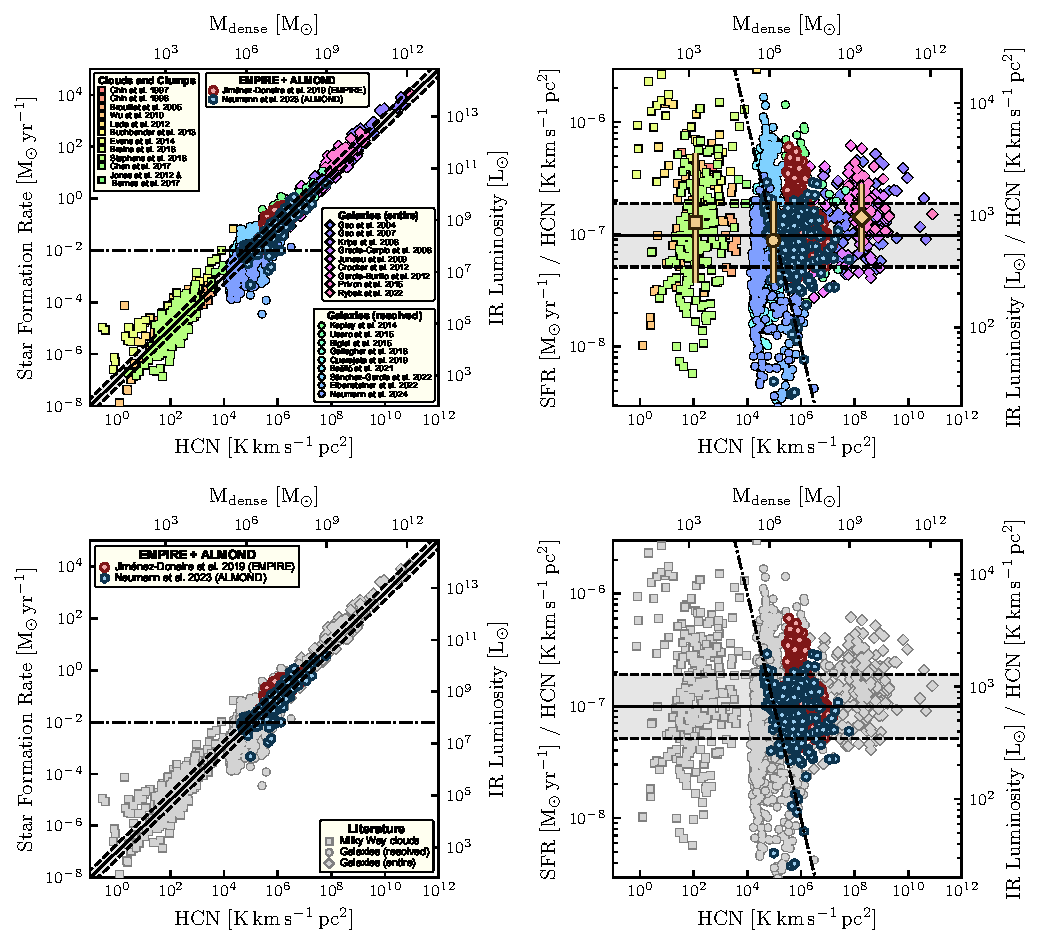
\includegraphics[width=\textwidth]{Figures/Gao_Solomon_relation_letter_compressed.pdf}
\caption{Gao--Solomon relation. Star formation rate (SFR, left) and star formation efficiency (SFE, right) of dense gas as a function of the HCN luminosity, tracing dense gas mass. Our literature compilation contains HCN observations that include Galactic clumps (squares), giant molecular clouds (GMCs), resolved nearby galaxies (circles) and unresolved entire galaxies (diamonds). 
Cloud- and clump-scale measurements are taken from observations within the Milky Way \citep{Wu2010, Lada2012, Evans2014, Stephens2016}, the CMZ \citep{Jones2012, Barnes2017} and the Local Group, i.e. \acrshort{lmc}/\acrshort{smc} \citep{Chin1997, Chin1998}, M31 \citep{Brouillet2005}, M33 \citep{Buchbender2013}, low-metallicity local group galaxies \citep{Braine2017}, and M51 \citep{Chen2017}.
Resolved galaxy observations, typically from nearby galaxies at $100\,$pc to $2\,$kiloparsec scales, include M82 \citep{Kepley2014}, M51 \citep{Usero2015, Querejeta2019}, NGC\,4038/39 \citep{Bigiel2015}, NGC\,3351, NGC\,3627, NGC\,4254, NGC\,4321, NGC\,5194 \citep{Gallagher2018a}, NGC\,3627 \citep{Beslic2021}, NGC\,1068 \citep{Sanchez-Garcia2022}, NGC\,6946 \citep{Eibensteiner2022}, NGC\,4321 \citep{Neumann2024}, and the two larger-sample surveys EMPIRE \citep[nine galaxies; ][]{Jimenez-Donaire2019} and ALMOND \citep[25 galaxies; ][]{Neumann2023a}.
Integrated-galaxy data cover LIRG/ULIRG and AGN galaxies \citep{Krips2008, Gracia-Carpio2008, Juneau2009, Garcia-Burillo2012, Privon2015}, early-type galaxies \citep{Crocker2012}, and high-redshift galaxies \citep{Gao2007, Rybak2022}.
The black solid line shows the median SFR/HCN computed from all data, with the dashed line marking the 1-sigma scatter (Tab.~\ref{tab:gao_solomon}). 
The large blue markers indicate the median values in the respective regimes. 
The bars in the right panel show the 16th-to-84th percentile range.}
\label{fig:gao_solomon_relation}
\end{figure*}
%-----------------------------------------------------------------

%-----------------------------------------------------------------
% GAO-SOLOMON TABLE
\begin{table}
    \begin{center}
    \caption{Gao--Solomon relation}
    \label{tab:gao_solomon}
    \resizebox{\columnwidth}{!}{
    \begin{tabular}{cccccc}
    \hline \hline
     & SFR/HCN & TIR/HCN & $\sigma$ & $\tau_{\rm dep}^{\rm dense}$ & $\epsilon_{\rm ff}^{\rm dense}$ \\
    \hline
    Clouds/Clumps	    & $-6.90$	& $2.93$	& $0.69$	& $8.07$	& $-2.43$ \\
    Resolved Galaxies	& $-6.99$	& $2.84$	& $0.37$	& $8.17$	& $-2.52$ \\
    Entire Galaxies	    & $-6.85$	& $2.98$	& $0.27$	& $8.03$	& $-2.38$ \\
    Combined	        & $-6.98$	& $2.85$	& $0.40$	& $8.15$	& $-2.51$ \\
     \hline\hline
    \end{tabular}
    }
    \end{center}
    {\bf Notes} -- Average dense gas scaling relation values across the combined literature sample presented in Fig.~\ref{fig:gao_solomon_relation} and for respective sub-samples, i.e. clouds/clumps, resolved and integrated galaxy surveys.
    All values are displayed on a logarithmic scale.
    Columns 2 and 3 list the average SFR/HCN and SFR/IR, using $\alphahcn=\SI{15}{\msun\per\square\parsec}\,(\SI{}{\kkms})^{-1}$.
    Column 4 shows the 1-sigma scatter ($\sigma$) of the detected data around the average value.
    Columns 5 and 6 display the dense gas depletion time (\taudense) and the dense gas star formation efficiency per free-fall time (\effdense).
\end{table}
%-----------------------------------------------------------------

%-------------------------------- Two column figure (place early!)
\begin{figure*}
\centering
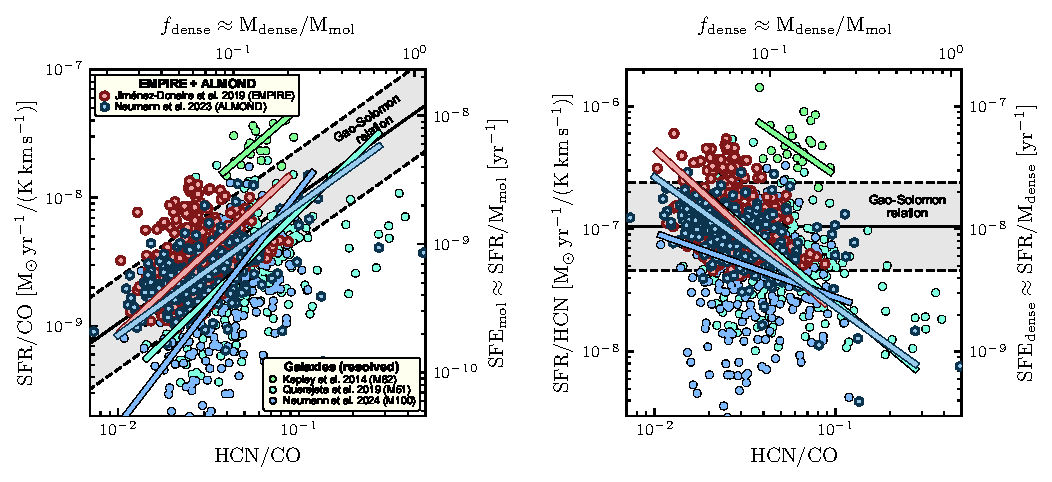
\includegraphics[width=\textwidth]{Figures/SFE_mol_and_dense_vs_fdense_relation_compressed.pdf}
\caption{Relations with HCN/CO as a proxy for the dense gas fraction. SFR-to-CO ratio (left) tracing the $\mathrm{SFE}_\mathrm{mol}$, and SFR-to-HCN ratio (right) tracing $\mathrm{SFE}_\mathrm{dense}$, as a function of the HCN-to-CO ratio, a proxy for the dense gas fraction. The colored circles represent measurements from EMPIRE (\citealp{Jimenez-Donaire2019}; red) and ALMOND (\citealp{Neumann2023a}; blue), as well as M82 measurements from \citet{Kepley2014} (blue), M51 from \citet{Querejeta2019} (green), and NGC\,4321 from \citet{Neumann2024}. The solid lines indicate the linear fits to the respective data.
}
\label{fig:hcn_ratio_relations}
\end{figure*}
%-----------------------------------------------------------------

% Two decades ago, \citet{Gao2004} found that HCN emission is tightly linked to the infrared luminosity in galaxies, proposing that HCN traces the dense gas that is intimately connected to the rate at which stars form, as opposed to the bulk molecular gas traced by CO.
% \citet{Wu2010}, \citet{Lada2012} and many others (see references in \ref{fig:dense:gs}) found a remarkably similar relation between HCN and IR luminosity within dense clumps of molecular clouds in the Milky Way, supporting a fundamental connection between dense molecular gas and star formation from sub-parsec to integrated-galaxy scales.
% Over the last twenty years, many more surveys aimed at mapping \hcnone in the local group and more recently across nearby galaxies at arcsecond relation, where ALMA has been a key player in efficiently mapping and resolving HCN in external galaxies at unprecedented resolution (references are listed in the text below).
% Today, we have an almost complete sampling of the HCN-IR plane from Milky Way clouds to distant galaxies (redshift $\leq 3$) spanning more than ten orders of magnitude.

In Fig.~\ref{fig:gao_solomon_relation}, we present the Gao--Solomon relation with one of the most complete and up-to-date compilations of HCN surveys with corresponding IR measurements\footnote{Note that some of the resolved HCN observations in nearby galaxies lack associated IR observations at a matched resolution \citep[e.g.,][]{Neumann2024} so that in these cases we rely on extinction-corrected \halpha observations to trace SFR.}.
The literature compilation comprises 31 HCN surveys from the Milky Way to the high-redshift universe.
The HCN surveys cover observations of molecular clouds within the Milky Way and the Local Group, spatially resolved measurements within galaxies and integrated intensity data, spanning scales from the solar neighbourhood to the distant, high-redshift universe (respective references are given in the figure caption).

On the $x$- and $y$-axes, we indicate the observed luminosities (HCN and IR) and the inferred physical quantities (\mdense and SFR) on secondary axes, assuming linear conversions with conversion factors $\alphahcn=\SI{15}{\msun\per\square\parsec}\,(\SI{}{\kkms})^{-1}$ from \citet{Schinnerer2024} and $\cir=\SI{1.48e-10}{\msun\per\year\per\lsun} = \SI{3.88e-44}{\msun\per\year}\,(\SI{}{\erg\per\second})^{-1}$ from \citet{Murphy2011}.
In the top right panel of Fig.~\ref{fig:gao_solomon_relation}, the $y$-axis displays the ratio between SFR and \lhcn (left axis) to highlight relative changes to a constant SFR/HCN.
The secondary $y$-axis shows the \lir-to-\lhcn ratio, which is proportional to SFR/HCN via the aforementioned \cir conversion factor. 
The black solid line in Fig.~\ref{fig:gao_solomon_relation} indicates the average SFR/HCN across the full literature sample and the grey shaded area represents the 1-sigma scatter of $\SI{0.40}{\dex}$.
We also compute the respective average \sfedense values and scatter ranges for the individual sample regimes, i.e. clouds (square), resolved galaxy observations (circle), and entire galaxies (diamond).
The values are listed in Tab.~\ref{tab:gao_solomon}.
Overall, the literature compilation demonstrates that the HCN luminosity is, to zeroth order, an excellent predictor of the star formation rate from cloud to galaxy scale, with consistent average \sfedense across 10 orders of magnitude.
However, the scatter increases from large ($\sigma=\SI{0.27}{\dex}$) to small scales ($\sigma=\SI{0.69}{\dex}$), indicating that variations within galaxies are larger than galaxy-to-galaxy variations.
This is already a first hint that there are systematic variations of \sfedense within galaxies (discussed in Sect.~\ref{sec:environment_relations}) that average out at integrated galaxy scales and that there might be other factors at play that affect \sfedense at kiloparsec to cloud scales.

In the bottom panels of Fig.~\ref{fig:gao_solomon_relation}, we show the same relations but specifically highlight data from EMPIRE (red) and ALMOND (blue), which are the two kiloparsec-scale resolved surveys of nearby galaxies featured in this work.
Both surveys roughly cover the same parameter space between $\lhcn=\SI{e4}{\kkms\square\parsec}$ and $\SI{e8}{\kkms\square\parsec}$, since they mapped the same type of spiral, star-forming galaxies at similar physical scales of $\sim$ kiloparsec.
It is shown that both data sets follow the Gao--Solomon relation and have comparable scatter, consistent with the full literature sample.
The resolution of $\sim$ kiloparsec is on the one hand high enough to resolve morphological structures like centres, bars and spiral arms and is on the other hand coarse enough to average over large enough regions to yield robust SFR measurements.
Therefore, this combined data set is the ideal sample to study resolved environmental trends of dense gas and star formation across nearby, star-forming galaxies.

The \sfedense tells us how many stars are forming per unit time per dense gas mass.
Assuming that the current amount of dense gas is causally linked to the currently measured SFR, \sfedense can be interpreted as the efficiency of converting dense molecular gas into stars.
In turn, assuming the current SFR stays constant over at least 100 million years, the inverse of \sfedense, i.e. the depletion time $\taudense=\mathrm{HCN/SFR}$ tells us how long it takes until the dense gas reservoir is completely converted into stars.
In this work, we find an average dense gas depletion time of $\langle\taudense\rangle=\SI{140}{\mega\year}$.
The star formation efficiency per free-fall time is given as $\effdense=\sfedense/\tffdense$, and takes into account the timescale of the gravitational collapse of the dense gas in the free-fall limit.
The free-fall time of the dense molecular gas (\tffdense) can be computed assuming that HCN traces gas above a density of $\ndense\approx \SI{e4}{\per\cubic\centi\metre}$.
Across the full literate sample, we obtain an average $\effdense=\SI{0.3}{\percent}$, which suggests that only \SI{0.3}{\percent} of the dense molecular gas is converted into stars.
This demonstrates that even in the dense, immediate star-forming gas, star formation appears to be an extremely inefficient process.


%-------------------------------- Two column figure (place early!)
\begin{figure*}
\centering
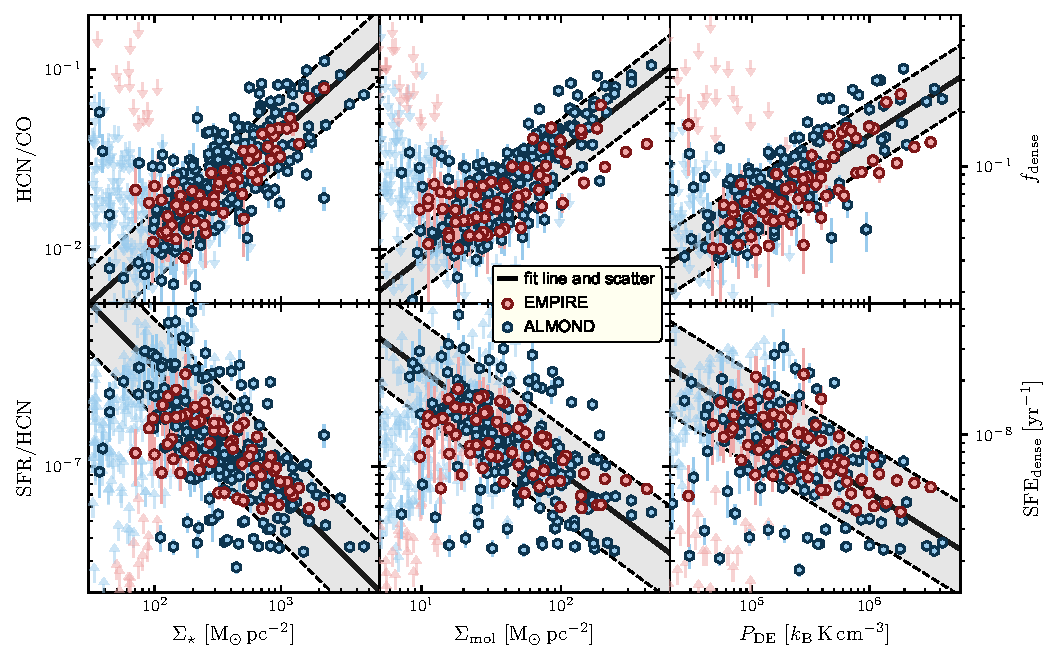
\includegraphics[width=\textwidth]{Figures/HCN_scaling_relations_compressed.pdf}
\caption{Dense gas relations with kiloparsec-scale environment. 
HCN/CO \textit{(top)}, a proxy of \fdense, and SFR/HCN \textit{(bottom)}, a proxy of \sfedense, as a function of stellar mass surface density (\sigstar), molecular gas surface density (\sigmol), and dynamical equilibrium pressure (\pde) across 31 galaxies from EMPIRE (red) and ALMOND (blue).
The markers denote significant ($\mathrm{S/N}\geq 3$) stacked measurements and the downward and upward pointing arrows indicate upper (HCN/CO) and lower limits (SFR/HCN).
All relations have been fitted with \texttt{LinMix} taking into account measurement uncertainties and upper/lower limits (parameters in Tab.~\ref{tab:environment}).
The black solid line shows the best fit line and the grey-shaded area indicates the 1-sigma scatter of the detected data.
}
\label{fig:environment_relations}
\end{figure*}
%-----------------------------------------------------------------

%-------------------------------------------------------------------
\subsection{Dense gas fraction relations}
%-------------------------------------------------------------------

The measured SFR/HCN yields consistently low dense gas star formation efficiencies across all surveys and scales.
However, there is a significant scatter of \sfedense about the mean relation.
In Fig.~\ref{fig:hcn_ratio_relations}, we present how \sfemol, traced by SFR/CO, and \sfedense, traced by SFR/HCN, vary with \fdense, traced by HCN/CO, across the EMPIRE and ALMOND galaxies, as well as within resolved measurement from the galaxies M51, M82 and NGC\,4321.
In each panel, we show the observationally-based ratios (HCN/CO, SFR/CO, SFR/HCN) on the primary $x$- and $y$-axes, and the inferred physical quantities (\fdense, \sfemol, \sfedense) on the secondary axes.
The physical quantities are computed assuming constant conversion factors, consistent with the values in Fig.~\ref{fig:gao_solomon_relation}.
% The dense gas fraction, \fdense, is assumed to be proportional to the HCN-to-CO line ratio:
% \begin{align}
% 	\fdense & =  \frac{\mdense}{\mmol} = \frac{\alphahcn \, \lhcn}{\alphaco \, \lco} \\
% 	\implies \fdense & = \num{3.45} \,\left(\frac{\lhcn}{\SI{}{\kkms\square\parsec}}\right) \left(\frac{\lco}{\SI{}{\kkms\parsec\squared}}\right)^{-1} \;.
% 	\label{equ:dense:fdense}
% \end{align}
% The star formation efficiency of the molecular gas, \sfemol, is traced via SFR-to-CO ratio:
% \begin{align}
% 	\sfemol & = \frac{\mathrm{SFR}}{\mmol} =  \frac{\mathrm{SFR}}{\alphaco\,\lco} \\
% 	\implies \left(\frac{\sfemol}{\SI{}{\per\year}}\right) & =  \num{2.30e-1}\,\left(\frac{\mathrm{SFR}}{\SI{}{\msun\per\year}}\right) \left(\frac{\lco}{\SI{}{\kkms\square\parsec}}\right)^{-1} \;.
% 	\label{equ:dense:sfemol}
% \end{align}
% Similarly, the SFR-to-HCN ratio is assumed to be proportional to the star formation efficiency of the dense gas:
% \begin{align}
% 	\sfedense & = \frac{\mathrm{SFR}}{\mdense} = \frac{\mathrm{SFR}}{\alphahcn\,\lhcn} \\
% 	\implies \left(\frac{\sfedense}{\SI{}{\per\year}}\right) & =  \num{6.67e-2}\,\left(\frac{\mathrm{SFR}}{\SI{}{\msun\per\year}}\right) \left(\frac{\lhcn}{\SI{}{\kkms\square\parsec}}\right)^{-1} \;.
% 	\label{equ:dense:sfedense}
% \end{align}

In agreement with previous works \citep[e.g.][]{Jimenez-Donaire2019}, we find that SFR/CO increases, while SFR/HCN decreases with HCN/CO across all surveys shown in Fig.~\ref{fig:hcn_ratio_relations}.
EMPIRE and ALMOND yield very similar relations that are also consistent with the higher resolution studies from M51 (at \SI{100}{\parsec}) and NGC\,4321 (at \SI{260}{\parsec}).
The starburst galaxy M82 shows significantly higher (factor of 3) SFR/CO and SFR/HCN at the same HCN/CO, indicating that starburst galaxies might be more efficiently producing stars.
Using the \texttt{BCES}\footnote{
% Bivariate Correlated Errors and intrinsic Scatter (BCES) is a generalisation of the ordinary least square fitting method developed by \cite{Akritas1996}, having the advantage of including measurement uncertainties on both coordinates and yielding proper orthogonal fit lines with reasonable uncertainty estimates. Here, we employ the \texttt{python} package from R. Nemmen: 
\url{https://github.com/rsnemmen/bces}} 
orthogonal best-fit lines, we obtain slopes between  $m=1.0$ (ALMOND) and  $m=1.8$ (NGC\,4321), where the kiloparsec-scale data (EMPIRE and ALMOND) yield slopes roughly consistent with a fixed SFR/HCN, i.e. the Gao--Solomon relation with a slope of 1 (black line in Fig.~\ref{fig:hcn_ratio_relations}).
Hence, the positive correlation between SFR/CO and HCN/CO suggests that clouds with a higher fraction of dense gas form stars more efficiently from the reservoir of bulk molecular gas, which is consistent with the picture that dense gas is the key ingredient to control star formation.
However, we also find that SFR/HCN systematically decreases with HCN/CO, finding slopes between $m=-0.53$ and  $m=-1.33$ in contradiction to a constant SFR/HCN.
If the physical quantities (\fdense and \sfedense) were taken at face value this would imply that denser clouds convert dense gas less efficiently into stars than less dense clouds.
An alternative interpretation put forward by e.g., \citet{Gallagher2018b} and \citet{Neumann2023a} is that at high HCN/CO, the molecular cloud density distribution is shifted to higher densities such that HCN is tracing more of the bulk molecular gas and not just the overdense gas, which is collapsing to eventually form stars.




%-------------------------------------------------------------------
\subsection{Dense gas relations with environment}
\label{sec:environment_relations}
%-------------------------------------------------------------------

%-------------------------------------------------------------------
% HCN/CO and SFR/HCN VS ENVIRONMENT FIT RESULTS
\begin{table}
\begin{center}
\caption{Dense gas scaling relations (environment)}
\label{tab:environment}
\resizebox{\columnwidth}{!}{
\begin{tabular}{cccccc}
\hline \hline
$\log_{10}(Y)$ & $\log_{10}(X)$ & $m$ (unc.) & $b$ (unc.) & $\sigma$ & Corr. ($p$)  \\
\hline
\multirow{3}{*}{HCN/CO}	& \sigstar	& $0.63$ $(0.03)$	& $-3.23$ $(0.07)$	& $0.19$	& $0.85$ $(\num{6.7e-120})$ \\
                        & \sigmol	& $0.60$ $(0.03)$	& $-2.65$ $(0.05)$	& $0.18$	& $0.87$ $(\num{9.7e-142})$ \\
                        & \pde	    & $0.42$ $(0.02)$	& $-3.86$ $(0.13)$	& $0.18$	& $0.83$ $(\num{6.9e-75})$  \\
\hline
\multirow{3}{*}{SFR/HCN}	& \sigstar	& $-0.70$ $(0.04)$	& $0.94$ $(0.10)$	& $0.27$	& $-0.76$ $(\num{7.4e-84})$ \\
                            & \sigmol	& $-0.57$ $(0.04)$	& $0.11$ $(0.07)$	& $0.26$	& $-0.75$ $(\num{9.1e-82})$ \\
                            & \pde 	    & $-0.41$ $(0.04)$	& $1.30$ $(0.19)$	& $0.26$	& $-0.68$ $(\num{3.2e-41})$ \\
 \hline\hline
\end{tabular}
}
\end{center}
{\bf Notes} --
Fit parameters obtained via linear regression with \texttt{LinMix} to the data shown in Fig.~\ref{fig:environment_relations}. $m$, $b$ and $\sigma$ are the slope, intercept and scatter of the relation.
Corr. ($p$) denotes the Pearson correlation coefficient with corresponding $p$--value.
\sigstar and \sigmol are given in units of \SI{}{\Msun\per\square\parsec}; and \pde in \SI{}{\kB\kelvin\per\cubic\centi\metre}.
\end{table}
%-------------------------------------------------------------------

%-------------------------------- Two column figure (place early!)
\begin{figure*}
\centering
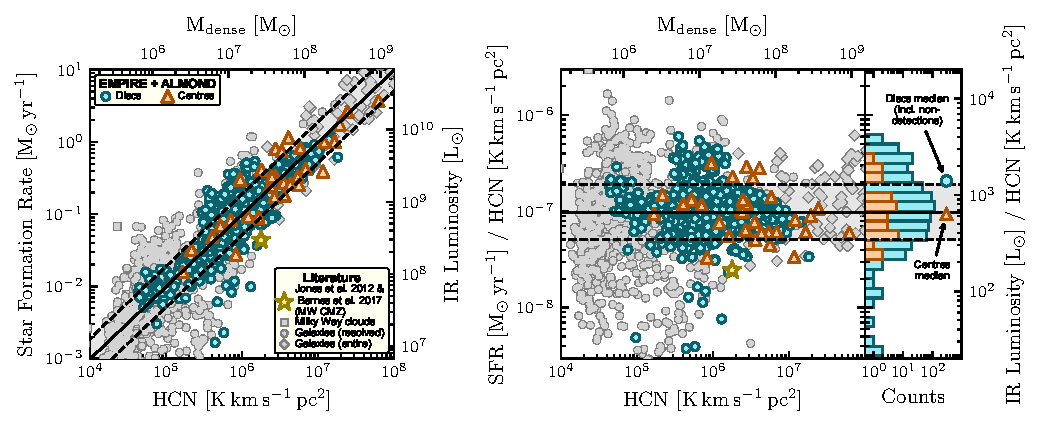
\includegraphics[width=\textwidth]{Figures/Gao_Solomon_relation_centres_compressed.pdf}
\caption{Gao--Solomon relation for galaxy centres. 
\textit{Left:} Similar to Fig.~\ref{fig:gao_solomon_relation}, but contrasting centres (orange triangles) and disc (cyan circles) measurements across the 31 galaxies from EMPIRE and ALMOND.
\textit{Right:} SFR/HCN against HCN for centres and disc, and additionally showing histograms of the detected centre (orange) and disc (cyan) data.
The markers (circle and triangle) in the histogram panel denote median SFR/HCN across the centres and discs, where also non-detections have to be taken into account.
}
\label{fig:centres}
\end{figure*}
%-----------------------------------------------------------------


Many previous works have found that HCN/CO and SFR/HCN are not constant within galaxies, but vary systematically with environmental properties.
\citet{Usero2015} and \citet{Gallagher2018a} show that HCN/CO systematically varies with the $\sim$ kiloparsec-scale, such as stellar surface density (\sigstar), molecular gas surface density (\sigmol), and environmental pressure (\pde).
\citet{Jimenez-Donaire2019} find similar positive correlations between HCN/CO and \sigstar, \sigmol, \pde and also report negative correlations between SFR/HCN and the aforementioned environmental conditions using the EMPIRE data.
Here, we present the best constraints on these scaling relations using the combined EMPIRE and ALMOND data (Fig.~\ref{fig:environment_relations}).
The physical quantities (\sigstar, \sigmol, \pde) are estimated as described in Sect.~\ref{sec:data}, using a constant \alphaco conversion factor to compute \sigmol and \pde.
The HCNone and \coone lines are spectrally stacked via  \texttt{PyStacker} (see e.g. \citetalp{Neumann2023b} for details on the spectral stacking methodology) via \sigstar, \sigmol and \pde for each galaxy individually using the \coone line as a prior.
For non-detected stacks, we provide upper (for HCN/CO) and lower limits (for SFR/HCN).
The relations are fitted to a linear function of the form:
\begin{align}
	\log_{10} Y = b + m \cdot \log_{10} X \;,
\end{align}
where $b$ and $m$ are the intercept and slope, and $Y=\{\mathrm{HCN/CO}, \mathrm{SFR/HCN}\}$ and $X=\{\sigstar, \sigmol, \pde\}$. 
The fitting is performed with the linear regression tool \texttt{LinMix}\footnote{
%\texttt{LinMix} uses a Bayesian approach to fit a line to data, taking into account censored data, measurement uncertainties and intrinsic scatter \citep{Kelly2007}. We employ the \texttt{python} package by J. Meyers: 
\url{https://github.com/jmeyers314/linmix}}
, which takes into account measurement uncertainties and censored data \citep[see e.g.][for more details on the fitting routine]{Neumann2023a}.
The fit parameters are presented in Tab.~\ref{tab:environment}.

We find similar scaling relations as reported by \citet{Jimenez-Donaire2019} but across a larger sample of galaxies and morphologies.
This means, HCN/CO increases, while SFR/HCN decreases with \sigstar, \sigmol, \pde.
However, there are some small differences compared to previous studies.
On the one hand, we find more significant fit relations due to the larger sample of galaxies, making the results reported in this work more robust.
On the other hand, we observe a larger scatter across the full sample of 31 galaxies compared to the EMPIRE galaxies alone, pointing towards galaxy-to-galaxy variations in the scaling relations.
The enhanced HCN/CO in high-surface density, high-pressure environments, could indicate that deeper gravitational potentials and higher external pressure exerted on molecular clouds lead to the formation of denser gas.
Furthermore, this denser molecular gas is less efficiently converted into stars since only the overdense part is expected to collapse and form stars \citep[based on turbulent cloud models, e.g., ][]{Krumholz2005}.
Overall, these results support the picture that there are consistent, systematic variations of HCN/CO and SFR/HCN with the$\sim$ kiloparsec-scale environment, suggesting that molecular clouds couple to the environment in which they are embedded.


%-------------------------------------------------------------------
\subsection{Dense gas relations in galaxy centres}
%-------------------------------------------------------------------

High-density, high-pressure regimes are typically found in centres of galaxies, hence one might expect systematically high HCN/CO and low SFR/HCN in galaxy centres compared to the discs.
In Fig.~\ref{fig:centres}, we separately show the centre measurements in contrast with the disc data in the Gao--Solomon relation.
For EMPIRE and ALMOND, the centres are simply a single sightline measurement from the centre of each galaxy and all remaining spaxels are denoted as disc environment.
To first order, we find that both environments (centres and discs) follow the Gao--Solomon relation with similar mean and scatter if purely based on detected measurement.
However, while the centre measurements are complete the disc data has a large fraction ($\sim\SI{80}{\percent}$) of non-detections.
To account for the non-completeness, we also compute the median SFR/HCN across the disc sightlines taking into account censored data, which yields $\mathrm{SFR/HCN}=\SI{2.1e-7}{\msun\per\year}\,(\SI{}{\kkms\square\parsec})^{-1}$, a factor of $2-3$ lower than the median across the centres ($\mathrm{SFR/HCN}=\SI{9.4e-8}{\msun\per\year}\,(\SI{}{\kkms\square\parsec})^{-1}$).
Hence, the typically higher density and pressure in galaxy centres appear to yield lower SFR/HCN.
We also measure a low SFR/HCN in the central molecular zone of the Milky Way, consistent with observations from nearby spiral galaxies.
If taken at face value, this would imply that galaxy centres are typically less efficiently forming stars per unit dense gas mass, which could be explained by higher gas turbulence in these environments acting against gravitational collapse.
However, we emphasise that especially galaxy centres are very complex regions and we might expect that \alphahcn varies between disc and centre regions, thus mitigating the interpretation of physical quantities like \mdense and \sfedense in galaxy centres.


%-------------------------------------------------------------------
\section{Conclusions}
\label{sec:conclusions}
%-------------------------------------------------------------------

This work studies $\sim$ kiloparsec-scale dense gas scaling relation using the newly acquired ALMOND dense gas survey from \citet{Neumann2023a}, which is supplemented by data from EMPIRE to form the largest resolved data set of dense gas maps from the nearby spiral galaxy population.
We find that the combined data set follows the well-established Gao--Solomon relation between SFR and HCN, demonstrating that, to zeroth order, HCN is linearly correlated with SFR over more than ten orders of magnitude, ranging from local clouds to the high-redshift universe, hence forming one of the most remarkable scaling relations in astronomy.
However, SFR/HCN (and HCN/CO) is not constant but varies systematically within galaxies as a function of environmental conditions measured on $\sim$ kiloparsec scales.
In this work, we provide the most robust constraints on these scaling relations using sensitive, stacked measurements across 31 galaxies, which show that HCN/CO increases and SFR/HCN decreases with stellar mass density, gas density, and external pressure.

In conclusion, this work shows that HCN/CO and SFR/HCN depend on $\sim$ kiloparsec-scale environment and \citet{Neumann2023a} find that these ratios also systematically vary with cloud-scale molecular gas properties.
Moreover, \citet{Sun2020a, Sun2020b} find that (using a similar sample of galaxies from PHANGS--ALMA) the properties of molecular clouds (surface density, velocity dispersion) are affected by the $\sim$ kiloparsec-scale environment
Linking these three findings, there is the emerging picture that the $\sim$ kiloparsec-scale environment controls the local conditions of molecular clouds, which in turn regulate the formation of dense gas and its subsequent conversion into stars.



%-------------------------------------------------------------------
\begin{acknowledgements}
LN acknowledges funding from the Deutsche Forschungsgemeinschaft (DFG, German Research Foundation) - 516405419.
AKL gratefully acknowledges support by grants 1653300 and 2205628 from the National Science Foundation, by award JWST-GO-02107.009-A, and by a Humboldt Research Award from the Alexander von Humboldt Foundation. The work of AKL is partially supported by the National Science Foundation under Grants No. 1615105, 1615109, and 1653300.
AU acknowledges support from the Spanish grants PGC2018-094671-B-I00, funded by MCIN/AEI/10.13039/501100011033 and by ``ERDF A way of making Europe'', and PID2019-108765GB-I00, funded by MCIN/AEI/10.13039/501100011033.

This paper makes use of the following ALMA data \\
% ALMOND
% PHANGS ALMA) CO(2-1)
ALMA is a partnership of ESO (representing its member states), NSF (USA), and NINS (Japan), together with NRC (Canada), NSC and ASIAA (Taiwan), and KASI (Republic of Korea), in cooperation with the Republic of Chile. The Joint ALMA Observatory is operated by ESO, AUI/NRAO, and NAOJ. The National Radio Astronomy Observatory (NRAO) is a facility of the National Science Foundation operated under cooperative agreement by Associated Universities, Inc.
\end{acknowledgements}
%-------------------------------------------------------------------

\bibliographystyle{aa}
\bibliography{references.bib}


%-------------------------------------------------------------------
\begin{appendix}
%-------------------------------------------------------------------


%-------------------------------------------------------------------
\section{Additional figures/tables}
\label{sec:app:fig_tab}
%-------------------------------------------------------------------

Tab.~\ref{tab:sample} presents the combined galaxy sample composed of 31 galaxies from the EMPIRE and ALMOND surveys, along with their coordinates and global properties.

%-------------------------------------------------------------------
\begin{table*}
\begin{center}
\caption{Galaxy sample (EMPIRE + ALMOND) \textcolor{red}{TBD: SOME VALUES MISSING}}
\label{tab:sample}
\resizebox{\textwidth}{!}{
\begin{tabular}{cccccccccccc}
    \hline\hline
    \multirow{2}{*}{Galaxy} & R.A. & Dec. & $d$ & $i$ & $M_\star$ & $M_{\htwo}$ & SFR & SFR/$M_\star$ & \multicolumn{2}{c}{Resolution} & \multirow{2}{*}{Survey} \\ 
    & (J2000) & (J2000) & ($\SI{}{\mega\parsec}$) & ($\SI{}{\degree}$) & ($\SI{e9}{\msun}$) & ($\SI{e9}{\msun}$) & ($\SI{}{\msun\per\year}$) & ($\SI{e-10}{\per\year}$) & ($\SI{}{\arcsecond}$) & (kpc) &  \\
    (1) & (2) & (3) & (4) & (5) & (6) & (7) & (8) & (9) & (10) & (11) & (12) \\
    \hline
    NGC\,0628 &   \ra{1;36;41.7} &   \ang{+15;47;1.1}   &   9.8 &   8.9 &   21.94 &   2.70 &   1.75 &       0.80 & 18.6 &        0.89 & ALMOND (EMPIRE) \\
    NGC\,1097 &   \ra{2;46;18.9} &  \ang{-30;16;28.8} &  13.6 &  48.6 &   57.48 &   5.52 &   4.74 &    0.83 & 19.4 &        1.28  & ALMOND \\
    NGC\,1365 &   \ra{3;33;36.4} &  \ang{-36;08;25.5} &  19.6 &  55.4 &   97.77 &  18.07 &  16.90 & 1.73 &  20.6 &        1.96 &  ALMOND \\
    NGC\,1385 &   \ra{3;37;28.6} &   \ang{-24;30;4.2} &  17.2 &  44.0 &    9.53 &   1.68 &   2.09 &      2.19 &  19.9 &        1.67  &  ALMOND \\
    NGC\,1511 &   \ra{3;59;36.6} &   \ang{-67;38;2.1} &  15.3 &  72.7 &    8.09 &   1.47 &   2.27 &        2.80 &  17.6 &        1.30  &  ALMOND \\
    NGC\,1546 &   \ra{4;14;36.3} &  \ang{-56;03;39.2} &  17.7 &  70.3 &   22.39 &   1.94 &   0.83 &   0.37 &  19.0 &        1.63  &  ALMOND \\
    NGC\,1566 &   \ra{4;20;0.4} &  \ang{-54;56;16.8} &  17.7 &  29.5 &   60.85 &   5.05 &   4.54 &    0.75 &  19.8 &        1.69  &  ALMOND \\
    NGC\,1672 &   \ra{4;45;42.5} &  \ang{-59;14;50.1} &  19.4 &  42.6 &   53.61 &   7.24 &   7.60 &     1.42 &  17.7 &        1.67  &  ALMOND \\
    NGC\,1792 &   \ra{5;05;14.3} &  \ang{-37;58;50.0} &  16.2 &  65.1 &   40.96 &   6.64 &   3.70 &    0.90 &  18.8 &        1.47  &  ALMOND \\
    NGC\,2566 &   \ra{8;18;45.6} &  \ang{-25;29;58.3} &  23.4 &  48.5 &   51.21 &   7.17 &   8.72 &     1.70 &  18.6 &        2.11  &  ALMOND\\
    NGC\,2903 &   \ra{9;32;10.1} &   \ang{+21;30;3.0} &  10.0 &  66.8 &   43.02 &   3.74 &   3.08 &     0.71 &  18.4 &        0.89  & ALMOND (EMPIRE)  \\
    NGC\,2997 &   \ra{9;45;38.8} &  \ang{-31;11;27.9} &  14.1 &  33.0 &   54.06 &   6.79 &   4.37 &      0.81 &  20.4 &        1.39  &  ALMOND \\
    NGC\,3059 &  \ra{9;50;8.2} &  \ang{-73;55;19.9} &  20.2 &  29.4 &   23.87 &   2.43 &   2.38 &     1.00 &  16.8 &        1.64  &  ALMOND \\\
    NGC\,3184 &  \ra{10;18;17.0} &  \ang{+41;25;28} &  13.0 & 16 & & & & & 33 & 2.07 &  EMPIRE \\
    NGC\,3521 &  \ra{11;05;48.6} &   \ang{-00;02;9.4} &  13.2 &  68.8 &  105.21 &   5.90 &   3.72 &    0.35 &  21.2 &        1.36  &  ALMOND \\
    NGC\,3621 &  \ra{11;18;16.3} &  \ang{-32;48;45.4} &   7.1 &  65.8 &   11.38 &   1.15 &   0.99 &       0.87 &  18.9 &        0.65  &  ALMOND \\
    NGC\,3627 &  \ra{11;20;15.0} &  \ang{+12;59;30} &  9.4 & 62 & & & & & 33 & 1.50  &  EMPIRE \\
    NGC\,4254 &  \ra{12;18;50.0} &  \ang{+14;24;59} &  16.8 & 32 & & & & & 33 & 2.68 &  EMPIRE \\
    NGC\,4303 &  \ra{12;21;54.9} &  \ang{+04;28;25.5} &  17.0 &  23.5 &   33.39 &   8.12 &   5.33 &   1.60 & 20.3 &        1.67   &  ALMOND \\
    NGC\,4321 &  \ra{12;22;54.9} &  \ang{+15;49;20.3} &  15.2 &  38.5 &   55.61 &   7.77 &   3.56 &    0.64 &  19.7 &        1.45  &  ALMOND (EMPIRE) \\
    NGC\,4535 &  \ra{12;34;20.3} &  \ang{+08;11;52.7} &  15.8 &  44.7 &   33.96 &   3.99 &   2.16 &   0.64 &  22.9 &        1.75  &  ALMOND \\
    NGC\,4536 &  \ra{12;34;27.1} &  \ang{+02;11;17.7} &  16.2 &  66.0 &   25.07 &   2.62 &   3.45 &     1.37 &  21.6 &        1.70  &  ALMOND \\
    NGC\,4569 &  \ra{12;36;49.8} &  \ang{+13;09;46.4} &  15.8 &  70.0 &   64.04 &   4.55 &   1.32 &   0.21 &  19.3 &        1.47  &  ALMOND \\
    NGC\,4826 &  \ra{12;56;43.6} &  \ang{+21;40;59.1} &   4.4 &  59.1 &   17.40 &   0.41 &   0.20 &      0.12 &  18.8 &        0.40  &  ALMOND \\
    NGC\,5055 &  \ra{13;15;49.2} &  \ang{+42;01;45}  & 8.9 & 59 & & & & & 33 & 1.42  &  EMPIRE \\
    NGC\,5194 &   \ra{13;29;52.7} &  \ang{+47;11;43} &  8.4 & 20 & & & & & 33 &  1.34 &  EMPIRE \\
    NGC\,5248 &  \ra{13;37;32.0} &   \ang{+08;53;6.7} &  14.9 &  47.4 &   25.49 &   4.54 &   2.29 &    0.90 &  19.9 &        1.44  &  ALMOND \\
    NGC\,5643 &  \ra{14;32;40.8} &  \ang{-44;10;28.6} &  12.7 &  29.9 &   21.69 &   2.66 &   2.59 &     1.20 &  18.1 &        1.11  &  ALMOND \\
    NGC\,6300 &  \ra{17;16;59.5} &  \ang{-62;49;14.0} &  11.6 &  49.6 &   29.45 &   1.90 &   1.89 &     0.64 &  17.7 &        1.00  &  ALMOND \\
    NGC\,6946 &  \ra{20;34;52.2} &  \ang{60;09;14} & 7.0 & 33 & & & & & 33 &  1.12 &  EMPIRE \\
    NGC\,7496 &  \ra{23;09;47.3} &  \ang{-43;25;40.3} &  18.7 &  35.9 &    9.92 &   1.81 &   2.26 &     2.28 &  17.9 &        1.63  &  ALMOND\\
    \hline\hline
\end{tabular}
}
\end{center}
\footnotesize{
    \textbf{Notes} -- (2) Right ascension, (3) declination, (4) distance \parencite[NASA Extragalactic Database (NED), or ][]{Anand2021}, (5) inclination angle \parencite{Makarov2014, Lang2020}.
    Integrated galaxy properties, (6) global stellar mass, (7) global H$_2$ mass and (8) global star formation rate are taken from \cite{Leroy2021b}.
    (10) native angular resolution, (11) corresponding linear resolution, given the distance $d$.
    (12) survey coverage.
}
\end{table*}
%-------------------------------------------------------------------


Tab.~\ref{tab:fdense} shows the SFR/CO, tracing \sfemol, and SFR/HCN, tracing \sfedense, versus HCN/CO, tracing \fdense, scaling relations measured from the different resolved galaxy surveys.

%-------------------------------------------------------------------
\begin{table*}
\begin{center}
\caption{Spectroscopic ratio relations}
\label{tab:fdense}
% \resizebox{\textwidth}{!}{
\begin{tabular}{ccccccc}
    \hline \hline
    $\log_{10}(Y)$ & $\log_{10}(X)$ & $m$ (unc.) & $b$ (unc.) & $\sigma$ & Corr. ($p$) & Reference  \\
    \hline
    \multirow{5}{*}{SFR/CO} & \multirow{5}{*}{HCN/CO} & $1.30$ $(0.05)$ & $-6.47$ $(0.08)$ & $0.16$ & $0.30$ $(\num{4.7e-09})$ & \cite{Jimenez-Donaire2019} \\ 
    &  & $1.02$ $(0.05)$ & $-7.03$ $(0.08)$ & $0.18$ & $0.44$ $(\num{5.2e-12})$ & \cite{Neumann2023a} \\ 
    &  & $1.23$ $(0.90)$ & $-6.06$ $(1.10)$ & $0.14$ & $0.25$ $(\num{2.3e-01})$ & \cite{Kepley2014} \\ 
    &  & $1.37$ $(0.09)$ & $-6.73$ $(0.12)$ & $0.21$ & $0.38$ $(\num{4.2e-10})$ & \cite{Querejeta2019} \\
    &  & $1.83$ $(0.13)$ & $-6.11$ $(0.19)$ & $0.21$ & $0.40$ $(\num{5.1e-12})$ & \cite{Neumann2024} \\ 
    \hline
    \multirow{5}{*}{SFR/HCN} & \multirow{5}{*}{HCN/CO} & $-1.33$ $(0.05)$ & $-9.02$ $(0.08)$ & $0.16$ & $-0.33$ $(\num{6.9e-11})$ & \cite{Jimenez-Donaire2019} \\
    &  & $-1.06$ $(0.06)$ & $-8.69$ $(0.10)$ & $0.17$ & $-0.51$ $(\num{2.0e-16})$ & \cite{Neumann2023a} \\ 
    &  & $-1.04$ $(1.02)$ & $-7.61$ $(1.23)$ & $0.15$ & $-0.24$ $(\num{2.5e-01})$ & \cite{Kepley2014} \\ 
    &  & $-1.23$ $(0.07)$ & $-8.83$ $(0.09)$ & $0.23$ & $-0.26$ $(\num{2.6e-05})$ & \cite{Querejeta2019} \\ 
    &  & $-0.54$ $(0.96)$ & $-8.10$ $(1.39)$ & $0.37$ & $-0.04$ $(\num{5.3e-01})$ & \cite{Neumann2024} \\
    \hline\hline
\end{tabular}
% }
\end{center}
\footnotesize{
\textbf{Notes} --
Fit parameters obtained via linear regression with \texttt{LinMix} to the data shown in Fig.~\ref{fig:hcn_ratio_relations}. 
$m$, $b$ and $\sigma$ are the slope, intercept and scatter of the relation.
Corr. ($p$) denotes the Pearson correlation coefficient with corresponding $p$-value.
}
\end{table*}
%-------------------------------------------------------------------




\vspace{10mm}
\noindent\textcolor{red}{\bf Ideas:}
\begin{itemize}
    \item \textcolor{red}{Variable \alphaco: show dense gas--environment relations (HCN/CO, SFR/HCN vs \sigmol and \pde) with variable \alphaco, using the best \alphaco prescription from PHANGS (probably then only for ALMOND); should make the point that slopes depend on methodology and can vary by $\sim$ factor of 2}
    \item \textcolor{red}{Spectra/intensity comparison between EMPIRE and ALMOND for the overlapping galaxies}
\end{itemize}



\end{appendix}

\end{document}


